\chapter{Adapter模式}
\section{适配器的概念}
\noindent\textbf{ 适配器模式(Adapter):}
将一个类的接口转换成客户希望的另外一个接口,使得原本由于接口不兼容而不能一起工作的那些类能一起工作。
\subsection{分类}
\begin{enumerate}
	\item 类结构型模式——使用继承
	\item 对象结构型模式——使用委托
\end{enumerate}
\textbf{注:}前者类之间的耦合度比后者高,且要求程序员了解现有组件库中的相关组件的内部结构,所以应用相对较少些。
\subsection{优点}
\begin{enumerate}
	\item 客户端通过适配器可以透明地调用目标接口;
	\item 复用了现存的类,程序员不需要修改原有代码而重用现有的适配者类;
	\item 将目标类和适配者类解耦,解决了目标类和适配者类接口不一致的问题。
\end{enumerate}
\subsection{缺点}
对类适配器来说,更换适配器的实现过程比较复杂。
\section{模式的结构}
类适配器模式可采用多重继承方式实现,如 C++ 可定义一个适配器类来同时继承当前系统的业务接口和现有组件库中已经存在的组件接口;Java 不支持多继承,但可以定义一个适配器类来实现当前系统的业务接口,同时又继承现有组件库中已经存在的组件。
\subsection{角色}
\begin{itemize}
	\item 目标(Target)接口:当前系统业务所期待的接口,它可以是抽象类或接口;
	\item 适配者(Adaptee)类:它是被访问和适配的现存组件库中的组件接口;
	\item 适配器(Adapter)类:它是一个转换器,通过继承或引用适配者的对象,把适配者接口转换成目标接口,让客户按目标接口的格式访问适配者。
	\item 请求者(Client):使用Target中方法。
\end{itemize}
\subsection{应用场景}
\begin{itemize}
	\item 以前开发的系统存在满足新系统功能需求的类,但其接口同新系统的接口不一致;
	\item 使用第三方提供的组件,但组件接口定义和自己要求的接口定义不同。
\end{itemize}
\subsection{结构图}
\begin{figure}[!h]
	\centering
	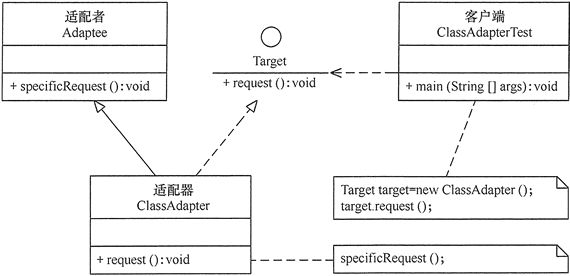
\includegraphics[width=0.8\textwidth]{image/2-1}
	\caption{类适配器模式的结构图}
\end{figure}
\begin{figure}[!h]
	\centering
	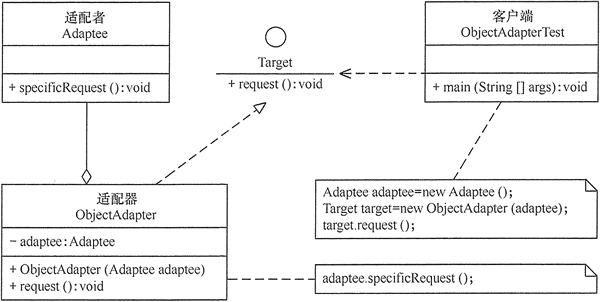
\includegraphics[width=0.8\textwidth]{image/2-2}
	\caption{对象适配器模式的结构图}
\end{figure}
\section{实现——例一}
\subsection{类适配器模式}
\begin{lstlisting}
//目标接口
interface Target {
	public void request();
}

//适配者接口
class Adaptee {
	public void specificRequest() {
		System.out.println("适配者中的业务代码被调用!");
	}
}

//类适配器类
class ClassAdapter extends Adaptee implements Target {
	public void request() {
		specificRequest();
	}
}

//客户端代码
public class ClassAdapterTest {
	public static void main(String[] args) {
		System.out.println("类适配器模式测试:");
		Target target = new ClassAdapter();
		target.request();
	}
}
\end{lstlisting}
\subsection{对象适配器模式}
\begin{lstlisting}
//目标接口
interface Target {
	public void request();
}

//适配者接口
class Adaptee {
	public void specificRequest() {
		System.out.println("适配者中的业务代码被调用!");
	}
}

class ObjectAdapter implements Target {
	private Adaptee adaptee;
	
	public ObjectAdapter(Adaptee adaptee) {
		this.adaptee = adaptee;
	}
	
	public void request() {
		adaptee.specificRequest();
	}
}

//客户端代码
public class ObjectAdapterTest {
	public static void main(String[] args) {
		System.out.println("对象适配器模式测试:");
		Adaptee adaptee = new Adaptee();
		Target target = new ObjectAdapter(adaptee);
		target.request();
	}
}
\end{lstlisting}
\section{实现——例二}
\subsection{类适配器模式}
\begin{lstlisting}
class Banner {
	private String string;
	
	public Banner(String string) {
		this.string = string;
	}
	
	public void showWithParen() {
		System.out.println("(" + string + ")");
	}
	
	public void showWithAster() {
		System.out.println("*" + string + "*");
	}
}

interface Print {
	public abstract void printWeak();
	public abstract void printStrong();
}

class ClassPrintBanner extends Banner implements Print {
	public ClassPrintBanner(String string) {
		super(string);
	}
	
	public void printWeak() {
		showWithParen();
	}
	
	public void printStrong() {
		showWithAster();
	}
}

public class ClassMain {
	public static void main(String[] args) {
		Print p = new ClassPrintBanner("hello");
		p.printWeak();
		p.printStrong();
	}
}
\end{lstlisting}
\subsection{对象适配器模式}
\begin{lstlisting}
class ObjectPrintBanner implements Print {
	private Banner banner;
		public ObjectPrintBanner(String string) {
		this.banner = new Banner(string);
	}
	public void printWeak() {
		banner.showWithParen();
	}
	public void printStrong() {
		banner.showWithAster();
	}
}

public class ObjectMain {
	public static void main(String[] args) {
		Print p = new ObjectPrintBanner("hello");
		p.printWeak();
		p.printStrong();
	}
}
\end{lstlisting}
\section{适配器扩展——双向适配器模式}
\begin{lstlisting}
//目标接口
interface TwoWayTarget {
	public void request();
}

//适配者接口
interface TwoWayAdaptee {
	public void specificRequest();
}

//目标实现
class TargetRealize implements TwoWayTarget {
	public void request() {
		System.out.println("目标代码被调用!");
	}
}

//适配者实现
class AdapteeRealize implements TwoWayAdaptee {
	public void specificRequest() {
		System.out.println("适配者代码被调用!");
	}
}

//双向适配器
class TwoWayAdapter implements TwoWayTarget, TwoWayAdaptee {
	private TwoWayTarget target;
	private TwoWayAdaptee adaptee;
	
	public TwoWayAdapter(TwoWayTarget target) {
		this.target = target;
	}
	
	public TwoWayAdapter(TwoWayAdaptee adaptee) {
		this.adaptee = adaptee;
	}
	
	public void request() {
		adaptee.specificRequest();
	}
	
	public void specificRequest() {
		target.request();
	}
}

//客户端代码
public class TwoWayAdapterTest {
	public static void main(String[] args) {
		System.out.println("目标通过双向适配器访问适配者:");
		TwoWayAdaptee adaptee = new AdapteeRealize();
		TwoWayTarget target = new TwoWayAdapter(adaptee);
		target.request();
		System.out.println("-------------------");
		System.out.println("适配者通过双向适配器访问目标:");
		target = new TargetRealize();
		adaptee = new TwoWayAdapter(target);
		adaptee.specificRequest();
	}
}
\end{lstlisting}
\begin{lstlisting}
//output
目标通过双向适配器访问适配者:
适配者代码被调用!
-------------------
适配者通过双向适配器访问目标:
目标代码被调用!
\end{lstlisting}
\begin{figure}[!h]
	\centering
	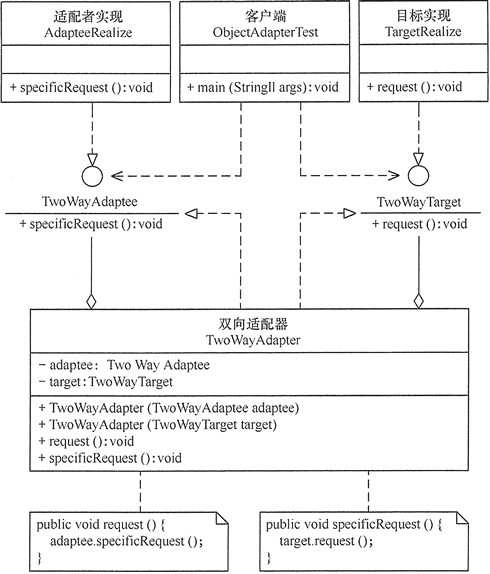
\includegraphics[width=0.8\textwidth]{image/2-3}
	\caption{双向适配器模式的结构图}
\end{figure}
\section{扩展思路}
\begin{enumerate}
	\item 什么时间使用Adapter?
	\subitem Adapter会将现有类适配,符合开闭原则,当出现bug时,可以明确知道不在现有Adaptee中。
	\item 使用适配器模式可以完全不改变现有代码前提下将代码适配于新的接口API,并非一定要现成的代码,可以随时编写。
	\item 版本升级可以使用适配器进行兼容。
	\item 当Adapter和Target角色功能完全不同时,Adapter模式不能使用。
	\item Adapter用于连接接口不同的类,Bridge用于连接类的功能层次结构与实现层次结构;
	\item Decorator不改变接口前提下增加功能,Adapter用于填补不同接口API之间缝隙。
\end{enumerate}

